
%% bare_jrnl.tex
%% V1.3
%% 2007/01/11
%% by Michael Shell
%% see http://www.michaelshell.org/
%% for current contact information.
%%
%% This is a skeleton file demonstrating the use of IEEEtran.cls
%% (requires IEEEtran.cls version 1.7 or later) with an IEEE journal paper.
%%
%% Support sites:
%% http://www.michaelshell.org/tex/ieeetran/
%% http://www.ctan.org/tex-archive/macros/latex/contrib/IEEEtran/
%% and
%% http://www.ieee.org/



% *** Authors should verify (and, if needed, correct) their LaTeX system  ***
% *** with the testflow diagnostic prior to trusting their LaTeX platform ***
% *** with production work. IEEE's font choices can trigger bugs that do  ***
% *** not appear when using other class files.                            ***
% The testflow support page is at:
% http://www.michaelshell.org/tex/testflow/


%%*************************************************************************
%% Legal Notice:
%% This code is offered as-is without any warranty either expressed or
%% implied; without even the implied warranty of MERCHANTABILITY or
%% FITNESS FOR A PARTICULAR PURPOSE!
%% User assumes all risk.
%% In no event shall IEEE or any contributor to this code be liable for
%% any damages or losses, including, but not limited to, incidental,
%% consequential, or any other damages, resulting from the use or misuse
%% of any information contained here.
%%
%% All comments are the opinions of their respective authors and are not
%% necessarily endorsed by the IEEE.
%%
%% This work is distributed under the LaTeX Project Public License (LPPL)
%% ( http://www.latex-project.org/ ) version 1.3, and may be freely used,
%% distributed and modified. A copy of the LPPL, version 1.3, is included
%% in the base LaTeX documentation of all distributions of LaTeX released
%% 2003/12/01 or later.
%% Retain all contribution notices and credits.
%% ** Modified files should be clearly indicated as such, including  **
%% ** renaming them and changing author support contact information. **
%%
%% File list of work: IEEEtran.cls, IEEEtran_HOWTO.pdf, bare_adv.tex,
%%                    bare_conf.tex, bare_jrnl.tex, bare_jrnl_compsoc.tex
%%*************************************************************************

% Note that the a4paper option is mainly intended so that authors in
% countries using A4 can easily print to A4 and see how their papers will
% look in print - the typesetting of the document will not typically be
% affected with changes in paper size (but the bottom and side margins will).
% Use the testflow package mentioned above to verify correct handling of
% both paper sizes by the user's LaTeX system.
%
% Also note that the "draftcls" or "draftclsnofoot", not "draft", option
% should be used if it is desired that the figures are to be displayed in
% draft mode.
%

\documentclass[11pt,draftclsnofoot,onecolumn]{IEEEtran}
%\documentclass[11pt,final,onecolumn]{IEEEtran}
%\documentclass[journal,twosides]{IEEEtran}
 \pagestyle{plain}
%
% If IEEEtran.cls has not been installed into the LaTeX system files,
% manually specify the path to it like:
% \documentclass[journal]{../sty/IEEEtran}





% Some very useful LaTeX packages include:
% (uncomment the ones you want to load)


% *** MISC UTILITY PACKAGES ***
%
%\usepackage{ifpdf}
% Heiko Oberdiek's ifpdf.sty is very useful if you need conditional
% compilation based on whether the output is pdf or dvi.
% usage:
% \ifpdf
%   % pdf code
% \else
%   % dvi code
% \fi
% The latest version of ifpdf.sty can be obtained from:
% http://www.ctan.org/tex-archive/macros/latex/contrib/oberdiek/
% Also, note that IEEEtran.cls V1.7 and later provides a builtin
% \ifCLASSINFOpdf conditional that works the same way.
% When switching from latex to pdflatex and vice-versa, the compiler may
% have to be run twice to clear warning/error messages.






% *** CITATION PACKAGES ***
%
\usepackage{cite}
% cite.sty was written by Donald Arseneau
% V1.6 and later of IEEEtran pre-defines the format of the cite.sty package
% \cite{} output to follow that of IEEE. Loading the cite package will
% result in citation numbers being automatically sorted and properly
% "compressed/ranged". e.g., [1], [9], [2], [7], [5], [6] without using
% cite.sty will become [1], [2], [5]--[7], [9] using cite.sty. cite.sty's
% \cite will automatically add leading space, if needed. Use cite.sty's
% noadjust option (cite.sty V3.8 and later) if you want to turn this off.
% cite.sty is already installed on most LaTeX systems. Be sure and use
% version 4.0 (2003-05-27) and later if using hyperref.sty. cite.sty does
% not currently provide for hyperlinked citations.
% The latest version can be obtained at:
% http://www.ctan.org/tex-archive/macros/latex/contrib/cite/
% The documentation is contained in the cite.sty file itself.






% *** GRAPHICS RELATED PACKAGES ***
%
\ifCLASSINFOpdf
  % \usepackage[pdftex]{graphicx}
  % declare the path(s) where your graphic files are
  % \graphicspath{{../pdf/}{../jpeg/}}
  % and their extensions so you won't have to specify these with
  % every instance of \includegraphics
  % \DeclareGraphicsExtensions{.pdf,.jpeg,.png}
\else
  % or other class option (dvipsone, dvipdf, if not using dvips). graphicx
  % will default to the driver specified in the system graphics.cfg if no
  % driver is specified.
  % \usepackage[dvips]{graphicx}
  % declare the path(s) where your graphic files are
  % \graphicspath{{../eps/}}
  % and their extensions so you won't have to specify these with
  % every instance of \includegraphics
  % \DeclareGraphicsExtensions{.eps}
\fi
% graphicx was written by David Carlisle and Sebastian Rahtz. It is
% required if you want graphics, photos, etc. graphicx.sty is already
% installed on most LaTeX systems. The latest version and documentation can
% be obtained at:
% http://www.ctan.org/tex-archive/macros/latex/required/graphics/
% Another good source of documentation is "Using Imported Graphics in
% LaTeX2e" by Keith Reckdahl which can be found as epslatex.ps or
% epslatex.pdf at: http://www.ctan.org/tex-archive/info/
%
% latex, and pdflatex in dvi mode, support graphics in encapsulated
% postscript (.eps) format. pdflatex in pdf mode supports graphics
% in .pdf, .jpeg, .png and .mps (metapost) formats. Users should ensure
% that all non-photo figures use a vector format (.eps, .pdf, .mps) and
% not a bitmapped formats (.jpeg, .png). IEEE frowns on bitmapped formats
% which can result in "jaggedy"/blurry rendering of lines and letters as
% well as large increases in file sizes.
%
% You can find documentation about the pdfTeX application at:
% http://www.tug.org/applications/pdftex





% *** MATH PACKAGES ***
%
%\usepackage[cmex10]{amsmath}
% A popular package from the American Mathematical Society that provides
% many useful and powerful commands for dealing with mathematics. If using
% it, be sure to load this package with the cmex10 option to ensure that
% only type 1 fonts will utilized at all point sizes. Without this option,
% it is possible that some math symbols, particularly those within
% footnotes, will be rendered in bitmap form which will result in a
% document that can not be IEEE Xplore compliant!
%
% Also, note that the amsmath package sets \interdisplaylinepenalty to 10000
% thus preventing page breaks from occurring within multiline equations. Use:
%\interdisplaylinepenalty=2500
% after loading amsmath to restore such page breaks as IEEEtran.cls normally
% does. amsmath.sty is already installed on most LaTeX systems. The latest
% version and documentation can be obtained at:
% http://www.ctan.org/tex-archive/macros/latex/required/amslatex/math/





% *** SPECIALIZED LIST PACKAGES ***
%
%\usepackage{algorithmic}
% algorithmic.sty was written by Peter Williams and Rogerio Brito.
% This package provides an algorithmic environment fo describing algorithms.
% You can use the algorithmic environment in-text or within a figure
% environment to provide for a floating algorithm. Do NOT use the algorithm
% floating environment provided by algorithm.sty (by the same authors) or
% algorithm2e.sty (by Christophe Fiorio) as IEEE does not use dedicated
% algorithm float types and packages that provide these will not provide
% correct IEEE style captions. The latest version and documentation of
% algorithmic.sty can be obtained at:
% http://www.ctan.org/tex-archive/macros/latex/contrib/algorithms/
% There is also a support site at:
% http://algorithms.berlios.de/index.html
% Also of interest may be the (relatively newer and more customizable)
% algorithmicx.sty package by Szasz Janos:
% http://www.ctan.org/tex-archive/macros/latex/contrib/algorithmicx/




% *** ALIGNMENT PACKAGES ***
%
%\usepackage{array}
% Frank Mittelbach's and David Carlisle's array.sty patches and improves
% the standard LaTeX2e array and tabular environments to provide better
% appearance and additional user controls. As the default LaTeX2e table
% generation code is lacking to the point of almost being broken with
% respect to the quality of the end results, all users are strongly
% advised to use an enhanced (at the very least that provided by array.sty)
% set of table tools. array.sty is already installed on most systems. The
% latest version and documentation can be obtained at:
% http://www.ctan.org/tex-archive/macros/latex/required/tools/


%\usepackage{mdwmath}
%\usepackage{mdwtab}
% Also highly recommended is Mark Wooding's extremely powerful MDW tools,
% especially mdwmath.sty and mdwtab.sty which are used to format equations
% and tables, respectively. The MDWtools set is already installed on most
% LaTeX systems. The lastest version and documentation is available at:
% http://www.ctan.org/tex-archive/macros/latex/contrib/mdwtools/


% IEEEtran contains the IEEEeqnarray family of commands that can be used to
% generate multiline equations as well as matrices, tables, etc., of high
% quality.


%\usepackage{eqparbox}
% Also of notable interest is Scott Pakin's eqparbox package for creating
% (automatically sized) equal width boxes - aka "natural width parboxes".
% Available at:
% http://www.ctan.org/tex-archive/macros/latex/contrib/eqparbox/





% *** SUBFIGURE PACKAGES ***
%\usepackage[tight,footnotesize]{subfigure}
% subfigure.sty was written by Steven Douglas Cochran. This package makes it
% easy to put subfigures in your figures. e.g., "Figure 1a and 1b". For IEEE
% work, it is a good idea to load it with the tight package option to reduce
% the amount of white space around the subfigures. subfigure.sty is already
% installed on most LaTeX systems. The latest version and documentation can
% be obtained at:
% http://www.ctan.org/tex-archive/obsolete/macros/latex/contrib/subfigure/
% subfigure.sty has been superceeded by subfig.sty.



%\usepackage[caption=false]{caption}
%\usepackage[font=footnotesize]{subfig}
% subfig.sty, also written by Steven Douglas Cochran, is the modern
% replacement for subfigure.sty. However, subfig.sty requires and
% automatically loads Axel Sommerfeldt's caption.sty which will override
% IEEEtran.cls handling of captions and this will result in nonIEEE style
% figure/table captions. To prevent this problem, be sure and preload
% caption.sty with its "caption=false" package option. This is will preserve
% IEEEtran.cls handing of captions. Version 1.3 (2005/06/28) and later
% (recommended due to many improvements over 1.2) of subfig.sty supports
% the caption=false option directly:
%\usepackage[caption=false,font=footnotesize]{subfig}
%
% The latest version and documentation can be obtained at:
% http://www.ctan.org/tex-archive/macros/latex/contrib/subfig/
% The latest version and documentation of caption.sty can be obtained at:
% http://www.ctan.org/tex-archive/macros/latex/contrib/caption/




% *** FLOAT PACKAGES ***
%
%\usepackage{fixltx2e}
% fixltx2e, the successor to the earlier fix2col.sty, was written by
% Frank Mittelbach and David Carlisle. This package corrects a few problems
% in the LaTeX2e kernel, the most notable of which is that in current
% LaTeX2e releases, the ordering of single and double column floats is not
% guaranteed to be preserved. Thus, an unpatched LaTeX2e can allow a
% single column figure to be placed prior to an earlier double column
% figure. The latest version and documentation can be found at:
% http://www.ctan.org/tex-archive/macros/latex/base/



%\usepackage{stfloats}
% stfloats.sty was written by Sigitas Tolusis. This package gives LaTeX2e
% the ability to do double column floats at the bottom of the page as well
% as the top. (e.g., "\begin{figure*}[!b]" is not normally possible in
% LaTeX2e). It also provides a command:
%\fnbelowfloat
% to enable the placement of footnotes below bottom floats (the standard
% LaTeX2e kernel puts them above bottom floats). This is an invasive package
% which rewrites many portions of the LaTeX2e float routines. It may not work
% with other packages that modify the LaTeX2e float routines. The latest
% version and documentation can be obtained at:
% http://www.ctan.org/tex-archive/macros/latex/contrib/sttools/
% Documentation is contained in the stfloats.sty comments as well as in the
% presfull.pdf file. Do not use the stfloats baselinefloat ability as IEEE
% does not allow \baselineskip to stretch. Authors submitting work to the
% IEEE should note that IEEE rarely uses double column equations and
% that authors should try to avoid such use. Do not be tempted to use the
% cuted.sty or midfloat.sty packages (also by Sigitas Tolusis) as IEEE does
% not format its papers in such ways.


%\ifCLASSOPTIONcaptionsoff
%  \usepackage[nomarkers]{endfloat}
% \let\MYoriglatexcaption\caption
% \renewcommand{\caption}[2][\relax]{\MYoriglatexcaption[#2]{#2}}
%\fi
% endfloat.sty was written by James Darrell McCauley and Jeff Goldberg.
% This package may be useful when used in conjunction with IEEEtran.cls'
% captionsoff option. Some IEEE journals/societies require that submissions
% have lists of figures/tables at the end of the paper and that
% figures/tables without any captions are placed on a page by themselves at
% the end of the document. If needed, the draftcls IEEEtran class option or
% \CLASSINPUTbaselinestretch interface can be used to increase the line
% spacing as well. Be sure and use the nomarkers option of endfloat to
% prevent endfloat from "marking" where the figures would have been placed
% in the text. The two hack lines of code above are a slight modification of
% that suggested by in the endfloat docs (section 8.3.1) to ensure that
% the full captions always appear in the list of figures/tables - even if
% the user used the short optional argument of \caption[]{}.
% IEEE papers do not typically make use of \caption[]'s optional argument,
% so this should not be an issue. A similar trick can be used to disable
% captions of packages such as subfig.sty that lack options to turn off
% the subcaptions:
% For subfig.sty:
% \let\MYorigsubfloat\subfloat
% \renewcommand{\subfloat}[2][\relax]{\MYorigsubfloat[]{#2}}
% For subfigure.sty:
% \let\MYorigsubfigure\subfigure
% \renewcommand{\subfigure}[2][\relax]{\MYorigsubfigure[]{#2}}
% However, the above trick will not work if both optional arguments of
% the \subfloat/subfig command are used. Furthermore, there needs to be a
% description of each subfigure *somewhere* and endfloat does not add
% subfigure captions to its list of figures. Thus, the best approach is to
% avoid the use of subfigure captions (many IEEE journals avoid them anyway)
% and instead reference/explain all the subfigures within the main caption.
% The latest version of endfloat.sty and its documentation can obtained at:
% http://www.ctan.org/tex-archive/macros/latex/contrib/endfloat/
%
% The IEEEtran \ifCLASSOPTIONcaptionsoff conditional can also be used
% later in the document, say, to conditionally put the References on a
% page by themselves.





% *** PDF, URL AND HYPERLINK PACKAGES ***
%
%\usepackage{url}
% url.sty was written by Donald Arseneau. It provides better support for
% handling and breaking URLs. url.sty is already installed on most LaTeX
% systems. The latest version can be obtained at:
% http://www.ctan.org/tex-archive/macros/latex/contrib/misc/
% Read the url.sty source comments for usage information. Basically,
% \url{my_url_here}.





% *** Do not adjust lengths that control margins, column widths, etc. ***
% *** Do not use packages that alter fonts (such as pslatex).         ***
% There should be no need to do such things with IEEEtran.cls V1.6 and later.
% (Unless specifically asked to do so by the journal or conference you plan
% to submit to, of course. )

\usepackage{graphicx}


\usepackage[caption=false,font=footnotesize]{subfig}
%\captionsetup[subfigure]{margin=0pt, justification=centering, singlelinecheck=false}
\graphicspath{{figures/}}
%\usepackage{subfigure}
%\usepackage{epstopdf}
\DeclareGraphicsExtensions{.pdf,.jpeg,.png}
\usepackage{morefloats}
\usepackage{amsmath}
\newtheorem{defn}{Definition}
%\newtheorem{prop}[defn]{Proposition}
\newtheorem{thm}{Theorem}
%\newtheorem{cor}[defn]{Corollary}
%\usepackage{algorithmic}
\usepackage{array}
%\usepackage{mdwmath}
%\usepackage{mdwtab}
%\usepackage{eqparbox}
\usepackage{url}
% \url{my_url_here}.
\usepackage{parskip}
%\setlength{\parskip}{\baselineskip}
\setlength{\parindent}{10pt}

% correct bad hyphenation here
\renewcommand{\baselinestretch}{1}
\hyphenation{op-tical net-works semi-conduc-tor pa-ckets}


\begin{document}
%
% paper title
\title{A Survey on AMI Communication Technologies and Routing Protocols in the NAN domain}
%
%
% author names and IEEE memberships
% note positions of commas and nonbreaking spaces ( ~ ) LaTeX will not break
% a structure at a ~ so this keeps an author's name from being broken across
% two lines.
% use \thanks{} to gain access to the first footnote area
% a separate \thanks must be used for each paragraph as LaTeX2e's \thanks
% was not built to handle multiple paragraphs
%

\author{Diego F. Ram\'{i}rez, 
			 Sandra~C\'{e}spedes\\%
			 Department of Information and Communications Technologies\\%
			 Icesi University, Cali, Colombia\\%
			 Email: \{\textit{dframirez,scespedes}\}\textit{@icesi.edu.co}}
% <-this % stops a space
%\thanks{D. Ram\'{i}rez and S. C\'{e}spedes are with the 
%Department of Information and Communication Technologies, Icesi University, Cali, Colombia. Email: \{dframirez,slcesped\}@icesi.edu.co}}%

% note the % following the last \IEEEmembership and also \thanks -
% these prevent an unwanted space from occurring between the last author name
% and the end of the author line. i.e., if you had this:
%
% \author{....lastname \thanks{...} \thanks{...} }
%                     ^------------^------------^----Do not want these spaces!
%
% a space would be appended to the last name and could cause every name on that
% line to be shifted left slightly. This is one of those "LaTeX things". For
% instance, "\textbf{A} \textbf{B}" will typeset as "A B" not "AB". To get
% "AB" then you have to do: "\textbf{A}\textbf{B}"
% \thanks is no different in this regard, so shield the last } of each \thanks
% that ends a line with a % and do not let a space in before the next \thanks.
% Spaces after \IEEEmembership other than the last one are OK (and needed) as
% you are supposed to have spaces between the names. For what it is worth,
% this is a minor point as most people would not even notice if the said evil
% space somehow managed to creep in.



% The paper headers
%\markboth{IEEE Transactions on Vehicular Technology,~Vol.~XX, No.~XX}{C\'{e}spedes \MakeLowercase{\textit{et al.}}: A Multi-hop Authenticated Proxy Mobile IP Scheme for Asymmetric VANET}
% The only time the second header will appear is for the odd numbered pages
% after the title page when using the twoside option.
%
% *** Note that you probably will NOT want to include the author's ***
% *** name in the headers of peer review papers.                   ***
% You can use \ifCLASSOPTIONpeerreview for conditional compilation here if
% you desire.




% If you want to put a publisher's ID mark on the page you can do it like
% this:
%\IEEEpubid{0000--0000/00\$00.00~\copyright~2007 IEEE}
% Remember, if you use this you must call \IEEEpubidadjcol in the second
% column for its text to clear the IEEEpubid mark.



% use for special paper notices
%\IEEEspecialpapernotice{(Invited Paper)}

% make the title area
\maketitle


\begin{abstract}

Smart Grid is defined as the modern infrastructure of the electric grid, whose objective is to improve efficiency, reliability, and security. This is achieved through the control automation of the transmission and distribution lines, the enhancement of consumption metering technologies, the implementation of new renewable energy sources and new energy management techniques. The growing demand of energy, changes in global weather, problems in the storing and distribution, and the need to implement more efficient consumption metering systems, are some of the factors that have led to transit towards a more complex and robust electric grid. A fundamental component of this new grid is an Advanced Metering Infrastructure (AMI), which provides a two-way communication flow between Utilities and meters and the customer side. In this paper we outline the main features of this new infrastructure, including communication technologies, topologies for deployment, and routing requirements in the Nighborhood Area Network (NAN) domain. For this purpose, we present the communication requirements for the AMI network (such as scalability, interoperability, latency,  security, quality of service, among others), and a full analysis of different routing strategies and protocols within the AMI context.
		

\end{abstract}
% IEEEtran.cls defaults to using nonbold math in the Abstract.
% This preserves the distinction between vectors and scalars. However,
% if the journal you are submitting to favors bold math in the abstract,
% then you can use LaTeX's standard command \boldmath at the very start
% of the abstract to achieve this. Many IEEE journals frown on math
% in the abstract anyway.

% Note that keywords are not normally used for peerreview papers.
\begin{IEEEkeywords}
AMI, AODV, DADR, DSR, Geographical Routing, HAN, HWMP, Mesh Under, NAN, PLC, Route Over, routing, Smart Grid, WiFi
\end{IEEEkeywords}






% For peer review papers, you can put extra information on the cover
% page as needed:
% \ifCLASSOPTIONpeerreview
% \begin{center} \bfseries EDICS Category: 3-BBND \end{center}
% \fi
%
% For peerreview papers, this IEEEtran command inserts a page break and
% creates the second title. It will be ignored for other modes.
\IEEEpeerreviewmaketitle


\section{Introduction}
\IEEEPARstart{S}{mart Grid} is defined as the modern infrastructure of the electric grid, whose objective is to improve efficiency, reliability, and security. This is achieved through the control automation of the transmission and distribution lines, the enhancement of consumption metering technologies, the implementation of new renewable energy sources, and the introduction of new energy management techniques \cite{Gungor2011}. The growing demand of energy, changes in global weather, problems in the storing and distribution, and the need to implement more efficient consumption metering systems, are some of the factors that have led to transit towards a more complex and robust electric grid. At the same time, the improvement in the response time to network faults, natural disasters, interference problems, and energetic resources loss, constitutes a strong reason to structure an electric grid with better energy transport, generation, and distribution technologies.

%On the other hand, due to the emerging energy crisis, caused by the depletion of fossil fuels and the corresponding reserves, global attention has been called to find alternative renewable energy sources, so that the industry can be sustained in the long term \cite{Wang2011a}. It is in this context that the concept of SG arises as a strategic solution to the energy optimization problem, since it is proposed that this new type of electric grid responds, in a dynamic and periodic way, to changes in the energy load that is being consumed. The new business model that now involves the client (who can be a consumer as well as a producer), would allow energy provision depending on climate changes, number of appliances switched on, and peak hours \cite{Castellani2012}. By these means, SG constitutes itself in the next generation of electric grid systems, that will incorporate different renewable energy resources, automatic and intelligent management of the energy and a more effective and interactive communication with the client.

 The electric grid transformation involves the integration of a bidirectional communication infrastructure. Regarding the distribution component of the electric grid, an advanced metering infrastructure (AMI), which results from the integration of advanced sensors, smart meters, monitoring systems, and energy management systems, has been a focus of interest for governments, utilities and academia. An initial implementation of the AMI involved the deployment of communication technologies to enable a two-way data flow for sending commands and information in real time to smart meters, as well as the reception of consumption information from the customer premises \cite{Deconinck2008}. Nowadays, it has been identified that the exchange of information between AMI devices will not be related exclusively to client's consumption, or the sending of control commands to smart meters. The list of applications is expanding to real time pricing, outage management, emergency response, in-home displays, among others \cite{Rajalingham2013}. Therefore, it is critical for the utilities to define the communications requirements and the more suitable technologies for implementing the bidirectional communication system. 
 
In this paper, we first identify the set of design factors that need to be considered in order to support the aforementioned applications in the AMI network. Since both wired and wireless technologies have been proposed for communications in the AMI, we survey the different communications technologies that have been proposed, with a focus on the network segment that connects the smart meters and data collectors, i.e., the Neighborhood Area Networks (NAN). Additional to communications technologies, we also survey and provide a  detailed description of the different routing protocols proposed for the NAN domain. The protocols are compared based on a set of metrics and the performance results reported in the literature. In our survey, we consider the fact that the chosen technology and routing protocol should adapt well to the kind of traffic that will be transmitted. Furthermore, the choice will be subject to other factors, such as the deployment time, the type of environment (rural/urban), and the operational costs of deployment and maintenance.

%In this article, we propose to outline the main features of the Advanced Metering Infrastructure (AMI), including communication technologies, topologies for deployment, and routing requirements. The overriding importance of the abovementioned subjects lies in the benefits that accrue for both Utilities and consumers, when enhancing the distribution system?s efficiency. On the one hand, Utilities will benefit from an automated information gathering system, reducing thus operational costs, as the system will collect and process data from the smart meters to its collectors located in strategic points within the service territory. Not only will the Utility benefit from an automated system for information gathering. A better understanding of how AMI works will allow utility to have a reduction in costs arising from lines losses (thefts and other kinds). On the other hand, users will have a better service experience as the two-way communication scheme enables a more interactive communication with the service provider. A decrease in operative costs and a better knowledge of their consumption patterns and electricity price in real time will also lead to reduced bills for residential and industrial customers. 

The remainder of this paper is organized as follows. In Section \ref{ami}, we describe the AMI network, its evolution regarding the AMI deployments reported around the world, and the design factors to consider at the time of deployment. In Section \ref{technologies}, we classify the communications technologies according to the network segment they fit better, and identify their advantages and disadvantages. Next, in Section \ref{routing} we provide the descriptions for the routing protocols proposed for the NAN domain, followed by Section \ref{metrics} with a qualitative comparison among the routing protocols. The open networking issues are described in Section \ref{issues}. Finally, concluding remarks are provided in Section \ref{conclusion}.

\section{Advanced Metering Infraestructure}\label{ami}

Smart grid communications comprise three types of networks: Home Area Networks (HAN), which serve as the communication infrastructure for sensors and devices inside homes; Neighborhood Area Networks (NAN), which connect smart meters and data collectors; and a Wide Area Network (WAN), which communicates data collectors with a utility control center  \cite{Tang2010}. The Advanced Metering Infrastructure (AMI) refers to the architecture that provides a two-way communication between the Utility and the Home Area Networks (HANs). It includes smart meters, a Meter Data Management System (MDMS), a communication network, access points, and a head-end  \cite{Wang2011b} \cite{Bennett2008}. An example of a typical AMI deployment is depicted in Fig. \ref{fig:ami}.

\begin{figure}[htp!]
\centering
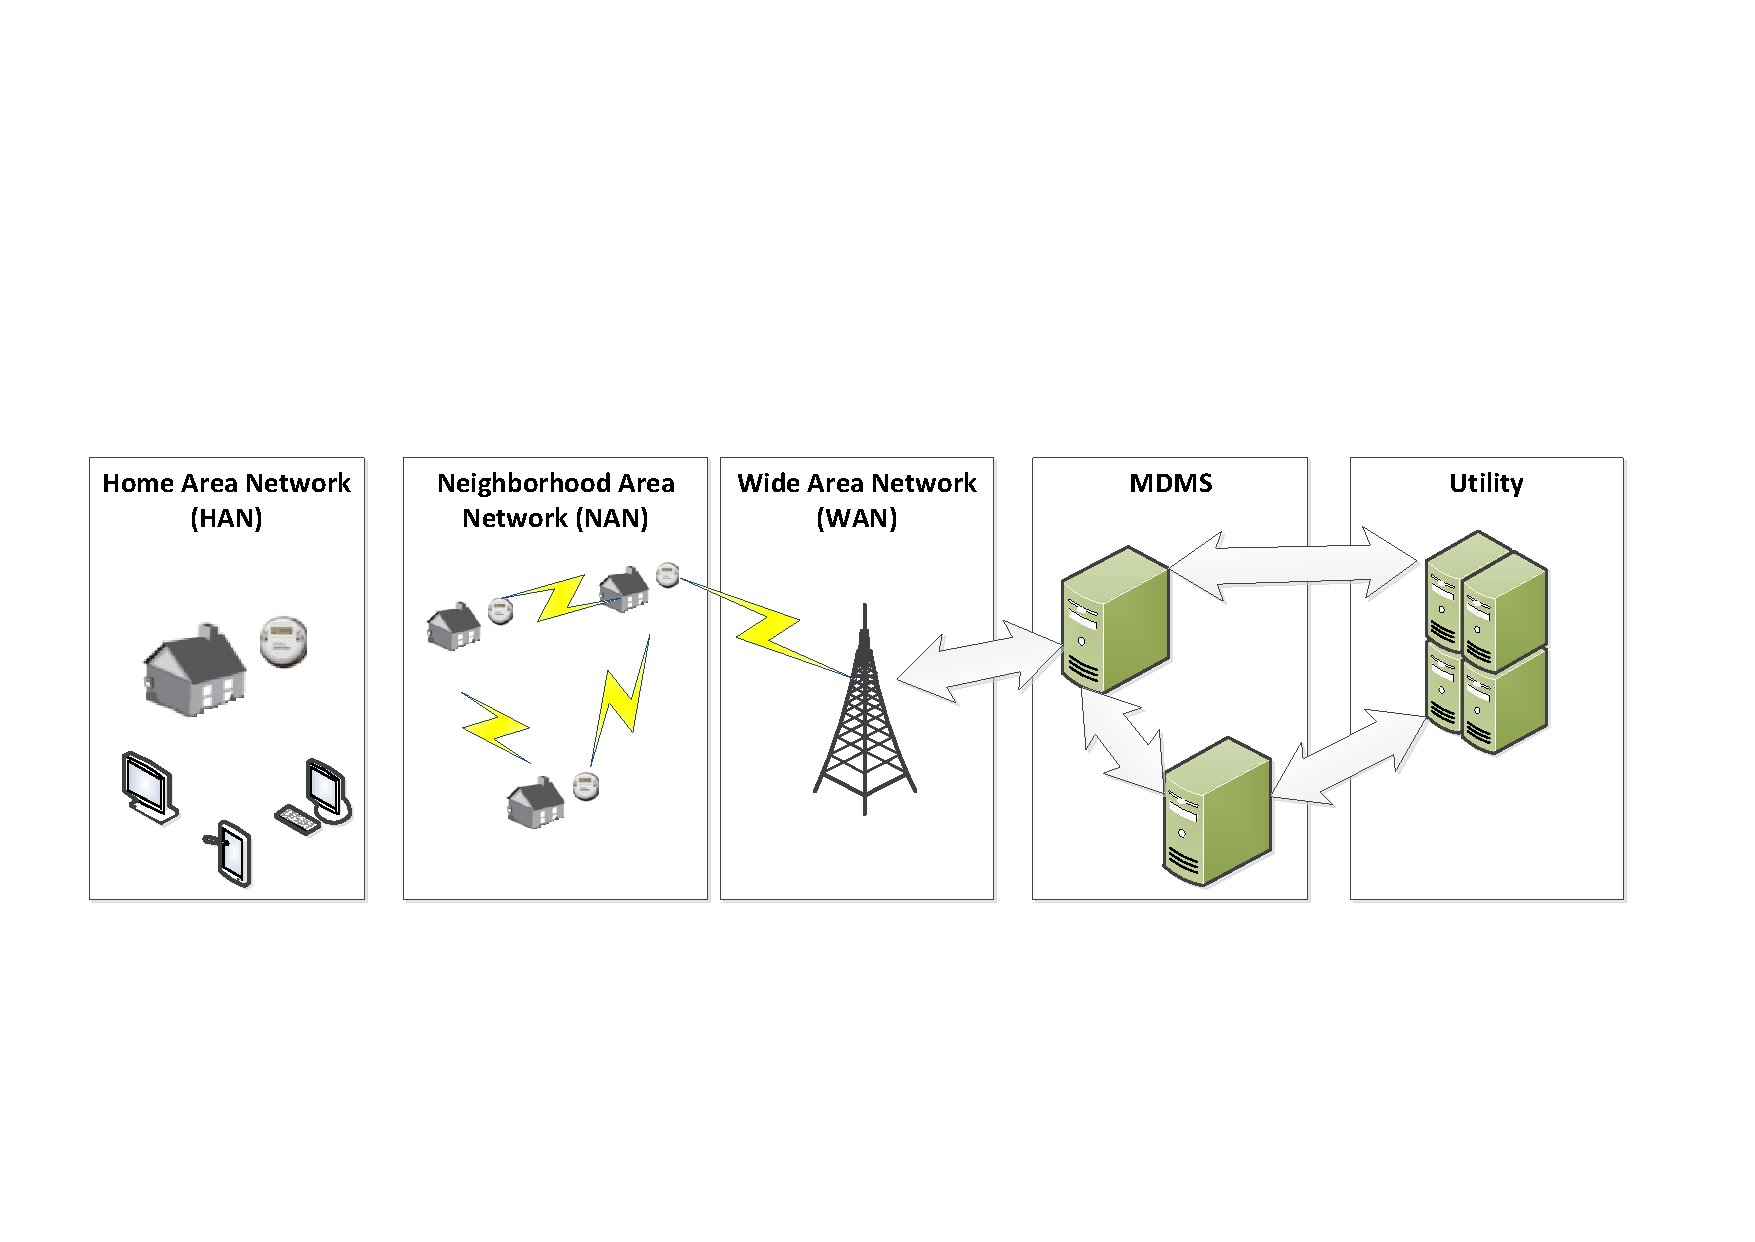
\includegraphics [height=12cm] {AMIArchitecture}
\caption{Basic AMI deployment}
\label{fig:ami}
\end{figure}

The main purpose of the AMI is to measure, gather, and analyze energy consumption as well as patterns of energy use.  The AMI must support  traffic generated at a variety of sources (meters, data collectors, and Utility). Therefore, the AMI network must fulfill %specific requirements to meet 
the needs of different natures of traffic while it may face constraints such as limited bandwidth and interaction with low-capacity devices (in terms of memory, processing capacity, and others).

While many utility companies started deploying AMI networks based on proprietary protocols, it is expected for the AMI communications architecture to be IP-based to guarantee interoperability with standard applications. As discussed by Yan \textit{et al.} \cite{Yan2013}, an IP-based network will provide an effective solution for the communication needs of the smart grid, as it becomes a non-technology dependant deployment.  Thus, the cost of implementation and maintenance can be reduced signifficantly using an IP-based approach. The main requirements for the IP-based communications network deployed in the AMI are as follows \cite{Wang2011b} \cite{Iyer2011a}:

\begin{itemize}
\item Interoperability: The IP suite and protocols should be standards-based with the purpose of enabling the communication between segments using different technologies and networking protocols, as well as providing end-to-end services.
\item Scalability: Supporting large and dense deployments is a must in the AMI network. 
\item Security: Smart meters transmit sensitive information on a regular basis; hence, the network must provide security for data transfer. Security services must cover different types of traffic and be provided at both network and application layers \cite{Bennett2008}. Real time information, for instance neighbors' energy consumption habits, become data that must be protected since third-party visibility of this information would constitute an invasion of privacy.
\item Reliability: It refers to the ability of the system to avoid, detect and repair eventual network faults. This involves avoiding data corruption, isolating faults in case of uncorrectable errors and eventually reporting them to recovery mechanisms.
\item Quality of Service: It refers to the ability of a system to provide different priority levels to different applications and types of traffic, so a certain level of performance of a data flow can be guaranteed.
\end{itemize}

An important aspect of the AMI's network operation is the routing of packets. The implementation of efficient routing strategies becomes paramount to guarantee that the information reaches its final destination. Therefore, routing protocols should be designed according to the aforementioned requirements. Furthermore, routing should be more or less robust, depending on the type of communication technology over which the AMI is deployed. In this article, we compare and discuss the routing strategies and protocols that have been adopted in the communications backbone of the AMI context.

\subsection{Overview of global deployment status of AMI}\label{ami}

The Advanced Metering and Demand Response Survey performed by FERC \cite{FERC2012} indicates that, in the U.S., the AMI penetration together with potential peak load reductions from electric power demand response have increased significantly since the last survey in 2008. The growth is around four percentage points (from 4.7\% in 2008 to 8.7\% in 2010). The study also shows that the Upper Midwest, West, and Texas have advanced metering penetration exceeding 13\%.

But not only the U.S shows a significant increase in AMI deployments. The European Union (EU) has set a target of 80\% smart meter deployment by 2020. However, there are still many questions to answer regarding demand response, off-peak usage, and planning for the deployment and support of electric vehicles. The main motivation in Europe for installing AMI appears to be limited to the operational efficiency of the Automatic Meter Reading (AMR) systems. However, due to the diversity of EU members and country-specific goals, the definition of a common AMI deployment methodology is a challenging task. Regarding the penetration of advanced metering approaches in Europe, countries such as Italy and Sweden have a near 100\% AMI implementation, but a large percentage of these deployments only have unidirectional communication capabilities (for AMR purposes). Functionalities such as demand response and load-shifting applications are restricted to larger customers  \cite{FERC2012}.

In Canada, the lasrgest AMI project in the region, called Hydro-Quebec, considers the deployment of four million smart meters. This is expected to be completed by 2017. As for Asia, China is on the way to expand their energy metering infrastructurein by promoting projects aimed at providing a two-way communication architecture between utilities and final consumers. Similarly, in Latin America, Brazil leads the AMI initiative by considering projects that contribute to the implemenation of a more automated metering approach, in the pursuit of investment recovery  \cite{Namboodiri2012}.


\subsection{Design Factors of the AMI Network}\label{designFactors}

Due to the evolution of the electrical grid, specifically electricity metering, a two-way communication network has been required. Applications such as smart metering, demand response (DR) and remote disconnect/reconnect require a communication network that supports them, as well as future application that will become prevalent, such as the sending of information about real time pricing from the Utility to the consumers homes or electric vehicles charging stations.  
Aspects regarding the choice of technology in which the AMI will be deployed, the constraints of the routing protocols, and the system capacity limits are some of the issues to solved through a proper network planning. This plan requires the use of best practice guidelines for the design and deployment of the AMI. The main factors to consider when designing AMI networks are outlined as follows \cite{Leon2011} :

\begin{itemize}
\item Understanding the networking needs and goals of the Utility
\item Identifying the main design constraints of the AMI vendor's equipment (in terms of hardware and software capacity).
\item Considering the compatibility with AMI communication protocols
\item Planning productions costs
\item Design of network topology, considering adaptability with wireless and wired communications
\item Identifying the need for pilot installation, field testing, and site infrastructure exploration
\item Developing a plan for deployment, testing, and post-design adjustments


\end{itemize}
		
Given that each Utility has different needs and expectations on the behavior of the AMI network, and considering the varying constraints on performance requirements, a fully understanding of these operation needs must be taken into account when designing the AMI. The design of the AMI Network should then consider all the factors described above, as they will define the approach to meet the Utility’s expectations.

In relation to the selection of vendors' equipment, the creation of link budgets for the various types of devices that will be used in the network deployment is the first step. In this processs, issues such as calculation of hopping limits, battery capacity limits and transmission power must be considered \cite{Leon2011}. Also, computer-aided design tools may be required for simulation, dimensioning and placement of infrastructure equipment purposes.  Through this kind of tools, the model of the network is created and then the planning of the whole system’s architecture can be deployed in the service area destined for that aim.

Another integral part in the design process is setting up a pilot system. In \cite{Leon2011}  a set-up of test transmitters in multiple locations within the service area is recommended. Execution of field measurements by testing the link configurations such as collector-to-meter, collector-to-repeater, and meter-to-meter is also proposed, in order to get a general view of the system performance.  

\section{Communication Technologies in AMI}\label{technologies}

In this section, we address the communication technologies suitable for AMI deployments. Although we introduce technologies related to the other domains in the smart grid (HAN and WAN), we devote a more detailed analysis for technologies in the NAN domain. 

\subsection{HAN domain}

\subsubsection{802.15.4-based technologies}\label{tech::802154}

The IEEE 802.15.4 standard specifies the physical and medium access control layers for Low Rate-Wireless Personal Area Networks LR-WPAN). The physical layer is divided in two layers: PHY data service and PHY management. The main function of the physical  layer is to transmit and receive messages through the radio medium. MAC layer provides two main services: MAC data service and MAC management service. Both of them allow the transmission and reception of frames through the PHY data service. Functions such as channel switching, energy detection measurement, clear channel assessment, security functions (AES encryption) and quality of service through guaranteed time slots are some of other features of this standard. Other technical characteristics of the 802.15.4 standard are listed below:

\begin{itemize}
	\item Frequency bands: 868 MHz/915 MHz and 2.4GHz
	\item Raw data rates: 868 MHz: 20kbps; 915 MHz: 40 kbps; 2.4GHz: 250 kbps
	\item Channels: 11 in the 868/915 MHz ; 16 in the 2.4 GHz
	\item Range: 10-20 m
	\item Latency: Down to 15ms
	\item Addressing: Short  8 bit or 64bit IEEE
	\item Channel access: CSMA-CA and slotted CSMA-CA
	\item Modulation technique: DSSS (Direct Sequence Spread Spectrum)
\end{itemize}  

One of the most well-known 802.15.4-based technologies is ZigBee \cite{Alliance2010}. It is a wireless communications technology considered ideal for real time monitoring of multiple targets, due to its low power consumption, low deployment cost, self-organization and self-configuration characteristics. As a result, ZigBee is especially useful in the HAN domain \cite{Sabbah2014}. Many AMI operators prefer smart meters on which the ZigBee protocol can be integrated, embracing the recommendation of the National Institute for Standards and Technology (NIST). Two different ZigBee specifications are available: \textit{i)} the one based on the RF4CE Specification, which is designed for running in low-power and resource-constrained devices, mostly for control applications. It employes specially-developed protocols for network and transport layers; and \textit{ii)} the IP-based version, named ZigBee IP, which provides mesh networking and IPv6 connectivity, enabling Internet access from ZigBee devices. The PHY and MAC layers of both specifications are based on the IEEE 802.15.4 standard.  

WirelessHART is another technology based on 802.15.4. This technology, however, defines Data Link, Network, and Transport layers for deploying real-time industrial control applications \cite{Song2008}. It has become very popular in the electric sector. In the link access, WirelessHART defines a 10ms time-slot for guaranteed link access. In the upper layers, it designates a centralized network manager in charge of maintaining updated routes. It also employs mesh-networking with self-healing and self-organizing characteristics.

There is also the possibility of employing standard Internet protocols directly over the 802.15.4 technology. 6LowPAN, a standard defined by the IETF, builds an adaptation layer between MAC layer and network layer to enable the transmission of IPv6 packets over IEEE 802.15.4 \cite{RFC4944}.  It describes the way packets of large sizes (i.e., IPv6 packets) can be transported through a wireless link that only accepts packets of a maximum 127 bytes size. For this purpose, header compression and fragmentation of IPv6 packets is performed, and mesh forwarding is also allowed for the delivery of packets from source to destination over multihop scenarios. Therefore, wireless embedded Internet access is enabled on any device, which provides an option for communications in HAN environments.
 
Among the advantages of technologies based on the 802.15.4 standard we can mention simplicity, robustness, low bandwidth requirements, low deployment cost, easy implementation, and the fact that they operate over a non-licensed spectrum band. They also allow for mobility of  devices. Regarding the drawbacks, one could mention the interference caused by other devices using the same transmission media, and the fact that technologies based on the 802.15.4 standard suffer from the scope expansion of sensor networks, the reason why these kind of technologies are only appropriate for small-scale networks deployments  \cite{Lu2011}.
 
 
% Main technical specifications, advantages and drawbacks of this technology are described below:
%
%Technical specifications: It has 16 channels in the 2.4GHz band, each with 5MHz bandwidth. Some of the values for the maximum power out of the radios in USA, Japan and Sweden are described as follows: The maximum power out of the radios with a transmission range between 1 and 100m is 0Dbm (1mW), with a data rate of 250 Kb/s, in OQPSK modulation \cite{Sabbah2014}

\subsubsection{802.11 and WiFi}

IEEE 802.11 standard \cite{Cali80211} specifies PHY and MAC layers for WiFi. It operates in the ISM 2.4 GHz. Tne IEEE 802.11b version of the standard is the one that has been widely adopted for WiFi. Main technical specifications of this standard are as follows:

\begin{itemize}
	\item Frequency bands: 2.4GHz
	\item Maximum data rate: 11 Mbps
	\item Channels: 13 overlapping 22 MHz wide frequency channels
	\item Range: 100 ft at 11 Mbps; 300 ft at 1 Mbps
	\item Channel access: CSMA-CA
	\item Modulation technique: DSSS)
\end{itemize}  

As WiFi is a very mature technology (it's estimated that more than 100 millon households worldwide have a WiFi installation for home networking) \cite{WiFi2010}, it becomes a suitable communication technology inside the HAN trhough wich devices at home send information to the smart meter. WiFi becomes a very scalable technology, providing extensive radio performance and network management mechanisms to provide records of radio quality, history reports and channel selection optimization. Regarding technical specifications, WiFi offers data rates from 1 Mbps (at 802.11b) to 600 Mbps (at 802.11n),  and support multichannels in the 2.4GHz and 5 GHz ISM bands. 

WiFi operates in unlicensed spectrum, so it's resilient to many types of interference but can coexist with other technologies that share this bands (it provides mechanisms to deliver robust performance in shared-spectrum and noisy RF environments  \cite{WiFi2010}). Other advantages of this technology include the fact that it enables IP-based applications, as it transports all IPv4 and IPv6-based protocols, the fact that many vendors implement the technology in a wide range of devices and enhancements in power management. As for the drawbacks, one could mention a higher power consumption (when compared with other HAN technologies such as ZigBee).  

\subsubsection{Ethernet}\label{ethernetl}

It is a very popular communication technology standard primarily used within the HAN, but can also be used on the NAN. A variety of speeds can be achieved, including 10Mbps, 100Mbps, 1000Mbps and 10000Mbps. Main advantages and drawdbacks are the following:

Advantages: Being standard-based, set up and configuration are easier.

Drawbacks: This technology may not be appropriate for connecting all devices in the HAN, due to the high cost and power requirements plus the need for separate cabling back to a central point.


\subsection{NAN domain}

\subsubsection{IEEE. 802.15.4g}\label{tech::802154g}

This is an amendment to the 802.15.4 standard whose objective is to facilitate very large scale process control applications such as the ones found in Smart Utility Networks. It is capable of supporting large and geographically diverse networks with minimal infrastructure and millions of fixed endpoints. The standard features an alternate PHY and the MAC modifications needed to support its implementation. The ammendment features the following \cite{Shin2010}:

\begin{itemize}

	\item Frequency bands: 700 MHz to 1GHz and the 2.4 GHz band.
	\item Frame Sizes: up to a minimun of 1500 octets
	\item It addresses SG geographic requirements by defining appropriate power levels
	\item It increases data rates formally to hundreds of kbps, and even Mbps, thus broadening the applicability of mesh systems beyond AMR and AMI to support the full sweep of smart grid applications. 
	\item The standard defines technologies supporting up to 1 Mbps
	\item It establishes a global standard by explicitly including unlicensed and region-specific frequency ranges, or spectrum bands
	\item It supports for Frequency Hopping Spread Spectrum (FHSS) transmission techniques.

\end{itemize}

It is natural that technologies based on the 802.15.4 standard (see Section \ref{tech::802154}) evolve to support the 802.15.4g technology, in order to provide communications for NAN environments. Such is the case for ZigBee, whose participation in standardization activities for smart grid NANs has been announced in early 2014. As for the advantages of the adoption of this standard, it provides backward compatibility built into the standard; thus, utilities' hardware can be integrated with no changes, so their investment in the technology is protected. IEEE 802.15.4g addresses reliability in outdoor environments, interference resiliency, and support of high density operation by FHSS techniques. The latter represents a vast improvement over historical not so reliable wireless technologies.

A summary of the technologies used in the HAN domain is depicted in  (Fig. \ref{fig:han}).

\begin{figure}[h!]
\centering
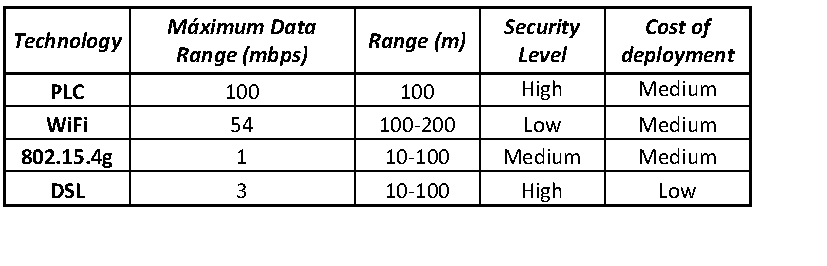
\includegraphics [height=15cm] {HAN-TECH}
\caption{Main technologies used in the HAN Domain}
\label{fig:han}
\end{figure}


\subsubsection{802.11s}\label{tech::80211s}

The IEEE 802.11s standard envisions a small-to medium- scale WLAN mesh network configured with a maximum of 32 mesh nodes (called Mesh Points MPs). An amendment to the standard has been made with the aim of developing a more flexible and extensible standard for wireless mesh networks based on IEEE 802.11. One of the most important functionalities of the new IEEE 802.11s is the multi-hop routing, which sets up the paths for the wireless forwarding. Mesh capabilities are provided to the mesh points, so they are able to participate in the forwarding process. Regarding the changes in this standard when compared with IEEE 802.11, the amendment is performed only in the MAC layer (modifications to PHY layer are not required) \cite{Bahr2006}.

\subsubsection{Power Line Communication (PLC)}\label{tech::plc}

PLC is a technology that uses the existing electric grid to transmit data. PLC becomes a well suited alternative as it is a no-cost medium for the Utility and is spread along the distribution system. Thus, PLC is a natural solution for the communication between the Utility and the Smart Meters. By reusing the electric grid as communication media, the implementation investment is low. In a typical PLC network, the smart meters are connected to the data center through power lines. The main technical specifications of this technology are stated below.

Two main types of communication architectures based on PLC have been defined: NarrowBand PLC (NBPLC) and Broadband PLC (BPLC). The first type allows data transmission at lower rates than those provided by BPLC (from few dozens of kbps to 100 Mbps, respectively) \cite{Sabbah2014}. NBPLC systems generally use the CENELEC (Comité Européen de Normalisation Electrotechnique) bands (3-148.5 kHz). NBPLC generally operates in transmission frequencies of up to 500 kHz, as opposed to BPLC, which targets much higher bandwidth at shorter distances and operates over a much higher frequency band. Frequencies of 148.5 kHz and less have been recognized by CENELEC standards for use in NBPLC systems on a public utility's power wires. Regarding the BPLC, the operation bands go from 1.8 MHz up to 250 MHz. Some examples of NBPLC technologies are described in IEEE 1901 and ITU-T G-hn (G.9960/G.9961) recommendations. NBPLC generally refers to PLC systems supporting data rates over 1 Mbps.

The main advantage of PLC is associated to the low implementation costs. Additionally, the coverage provided by PLC is exactly the one intended by the Utility. As it uses the power feeder, PLC behaves as an enabler for sensing, control, and automation in large systems comprising tens or even hundreds of components spread over relatively wide areas, which contributes to provide scalability. Furthermore, as the power lines are owned by the Utility, there is more independence in relation to sending information through third-party networks or operators. Nonetheless, the very nature of  PLC's physical transmission media generates some challenges. It is highly susceptible to signal degradation due to the harsh power lines. The technology is also limited by its low bandwidth, which is why it may not be suitable for more robust applications where large amounts of data need to be transferred. Besides the fact that feeder cables are not designed for data transmission, they are also prone to be interfered by the inverter’s outcome. %Therefore, PLC modems developed for domestic applications may not be suitable. 

A summary of the technologies used in the NAN domain is depicted in (Fig. \ref{fig:nan}).

\begin{figure}[h!]
\centering
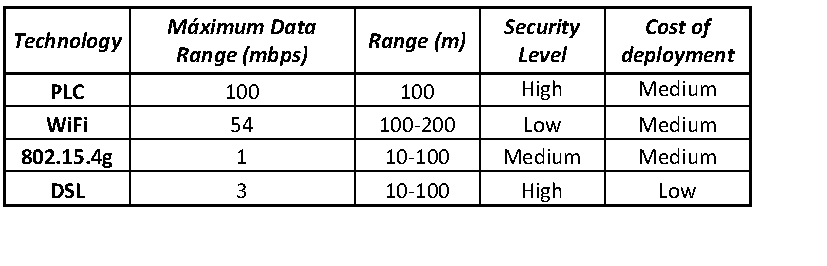
\includegraphics [height=15cm] {NAN-TECH}
\caption{Main technologies used in the NAN Domain}
\label{fig:nan}
\end{figure}


\subsubsection{Digital Subscriber Lines (DSL)}\label{dsl}
DSL is a high speed digital data transmission technology, which employs the wires of the voice telephone network for data transmission. As with PLC, this technology may be a suitable candidate for the implementation of network segments within the AMI, as it reuses the existing infrastructure, thus reducing installation cost of an implementation from scratch. As for the technical specifications, the network performance and perceived throughput will depend on how far away the subscriber is from the serving telephone  \cite{Gungor2011}. Main technical details, advantages and drawbacks of this technology are listed below:

Technical specifications: Commonly, the frequencies on which this technology works are greater than 1MHz through an ADSL enabled telephone line. 

As for the advantages of this technology, one coud mention that given a high data transmission rate and the low installation costs for the network deployment, DSL is a good option for the AMI implementation. Regarding the drawbacks, distance dependency is the primary constraint of this technology.

\subsection{WAN domain}

\subsubsection{Cellular Networks}\label{tech::cellular}
Cellular Networks became a popular technology for the communication between meters and the Utility, as a solution for Automatic Meter Reading systems. By employing short messaging services (SMS) or data plans through a cellular operator, the AMR system is supported over existing infrastructure, thus avoiding incurring in additional installation and deployment costs from the Utility's viewpoint. Furthermore, this technology is also suitable for communicating collectors to the central data center at the Utility's premises. Some of the cellular technologies employed for the long-haul communication are: 2G, 2.5G, 3G, and LTE. The latter has a high-capacity of bandwidth and, consequently, can also support several QoS requirements.

Among the advantages of employing this technology we can mention that by outsourcing the communications network to a mobile operator, utilities can significantly reduce operative costs, as they do not have to bear the cost of deploying and maintaining the infrastructure. Data rates for cellular technologies in AMI projects are now much more competitive. Furthermore, coverage provided by cellular networks is another outstanding advantage, which helps to improve network capabilities. On the contrary, among the drawbacks identified are those associated to information security. As the physical medium used for transmission is susceptible to interceptions, sensitive information (such as contractual data or bills) must be protected, to guarantee that it reaches its intended recipient with no understanding by other individuals or devices attempting to intercept it. In addition, given that the communication channel is shared with mobile telephony users, the network performance may be impaired at certain times or places. Moreover, transmission through cellular networks still has a high cost, especially when SMS is used as communication media between smart meters and data collectors. 


\subsubsection{WiMAX}\label{tech::wimax}

Wimax (Worldwide Interoperatibility for Microwave Access) is a wireless broadband technology based on the standard IEEE 802.16 \cite{IEEE80216}. One of the main characteristics of Wimax is that its adaptive modulation and coding scheme allows the whole network to adjust signal  modulation or coding depending on how noisy the link is. This is why the technology provides high data rates, as the modulation increases when signal to noise ratio is also increasing. Some technical specifications of the technology are \cite{Aguirre2013}:

\begin{itemize}

	\item Data rates: up to 70 Mbps
	\item Not protocol-dependent
	\item Low latency: <100 ms round trip
	\item It supports QoS, policy and traffic management
	\item It provides secure communication and provides 128 -bit Advanced Encryption Standard (AES)

\end{itemize}

Regarding the advantages of Wimax as  technology enabling communications in the NAN domain, one could focus mainly in the fact that it provides a balance between deployment cost, complexity, flexibility, and control. Being based on a flat architecture, the technology is flexible and scalable. On the other hand, it can use a wide range of frequencies and htis gives Utilities the possibility to deploy a wide range of applications with different bandwidth requirements and priority levels \cite{Senza2010}. As for the drawbacks, while Wimax provides a solution with a large communication range and high data rates, it tends to be costlier due to the greater licensing and subscription fees.


\section{Routing for Neighborhood Area Networks in AMI} \label{routing}

The Advanced Metering Infrastructure (AMI) is expected to be deployed on networks with a dense number of nodes (meters) that connect to numerous data collectors. Furthermore, the AMI network should provide efficient and suitable routing functionalities, which guarantee a reliable and effective delivery of information. Regarding the traffic involved in the two-way communication channel, different types of traffic can be identified: 1) traffic consisting of data containing the meter-reading, going from homes to Utilities’ data collectors, 2) traffic consisting of data containing data going from collectors to substation or the Utility itself, and 3) traffic consisting of data from applications in the Smart Grid. Some of these applications are \cite{Tan2011}: lighting control, heating, ventilation, detection of fluctuations and power outages, switchin on and off (remote control of the meter from customer side), demand response and vehicle charging. 

Considering the the importance behind the implementation of efficient routing strategies and protocols lies in the need of an effective data packet delivery mechanism, we foucse on the routing for the NAN domain the AMI architecture. As it is required that information from data collectors can be successfully received by the Utility, through the bidirectional communication channel outlined under the AMI concept, and conversely information from Utility must reach data collector and meters at the customer side, we analyse several routing protocols that have been proposed for the NAN domain. In \cite{Sabbah2014} several routing protocols have been classified and evaluated according to a certain set of metrics that will further be explained. 

\subsection{RPL}\label{rpl}

In an AMI network, the routing protocol must guarantee low energy consumption, assure privacy and information security, as well as support self-organization and self-configuration features. For this purpose, the IETF has proposed the Routing Protocol for Low Power and Lossy Networks \cite{Winter2012}. This protocol is of the distance-vector type, and is based on IPv6. It was designed considering the requirements specified in RFC 5826 \cite{Brandt2010}, RFC 5673 \cite{Pister2009}, RFC 5548 \cite{Dohler2009} and RFC 5867 \cite{Martocci2010}. Some of these requirements include: i) Scalability, which refers to the capability of supporting the organization of a large number of nodes into areas of configurable size; ii) Dinamicity, which makes reference to the capability of the routing protocol to support updating mechanisms in order to be informed of changes of connectivity, facitilitating reorganization and self-healing features; iii) Latency, which refers to how long it takes for a packet to get from source to destination throughout the network; and iv) ParameterConstrained Routing, which has to do with identifying node capabilities that will be used by the routing protocol for forwarding decision (e.g. CPU, memory size, battery level, etc.).

One of the main advantages of this protocol is that it does not define a unique routing metric, but gathers a set of metrics. This is a must in the AMI network, given its heterogeneous and diverse traffic natures. Multiple devices involved in the AMI, as well as the different types of applications uploaded to the network, entails a need to define several types of metrics to ensure the protocol efficiency. An objective function (OF) is defined for the purpose of combining a set of metrics. The main idea behind RPL is to maintain information about the network status using one or more directed acyclic graphs (DAGs). A DAG is a directed graph in which all edges are oriented in such a way that no cycles exist. For each DAG created in RPL there is a root. The DAG’s root is typically the gateway in the AMI network. All edges in the DAG are contained in the routes oriented to the root node. Each node in the DAG is associated to a rank. For the construction of the DAG, the gateway creates control messages called DIOS (DAG Information Object). The main functions executed by the DIO messages are listed below  \cite{Iyer2011a}:

\begin{itemize}
	\item To identify the DAG from which any root is originated
	\item To spread the Rank information of the starting node
	\item To define the objective function (OF) that specifies the metric, or the combination of metrics, used to compute the rank in each node.
\end{itemize}

Once multiple DIO messages have been received, a node computes its own rank and determines its position in the DAG. One way to compute the rank is utilizing the Expected Transmission Count (ETX) as a metric. ETX measures the quality of a route between two nodes, by estimating the average number of required transmissions to send data packets to a neighbor. Since nodes in a network are susceptible to multiples faults, RPL builds a Destination Oriented DAG (DODAG) with several routes from each node. This contributes to enhance the performance and robustness of the network, as well as to guarantee quality of service and to handle traffic in real time  \cite{Pavkovic2011}.

A detailed implementation of RPL for AMI networks is presented in \cite{Wang2010}. The authors considered a static multi-hop wireless AMI network that consists of \textit{n} meter nodes and one gateway node. In the proposed protocol, a DAG structure is maintained at the gateway node. Once the information that must be stored and maintained by each node is defined, the data traffic forwarding rules are introduced. The authors also provide a detailed characterization for the DAG construction and maintenance, and propose a reverse path recording mechanism in order to enable routing support for outward unicast traffic, which flows from the gateway to each meter. The practical implementation of RPL presented by Wang \textit{et al.} aims at providing reliable and low-latency routing support for large-scale AMI networks, through the integration with CSMA-based MAC layer protocols. 

\subsection{Geographic routing}\label{geographic}

Geographic routing considers packet forwarding by means of position information instead of network addresses and routing tables. The destination location is employed to route packets. Through the knowledge of neighbors' locations, each node selects the next hop that is closer to the destination. Regarding the determination of every node's position, GPS devices are the main tool for making position information available. In order to enable the node's awareness of its neighbors' positions, it is required the broadcasting of the position information to other nodes. To determine the position of the destination, a location service that maps network addresses to geographic locations is needed. 

One of the main advantages of this routing protocol is that routing tables maintenance and route discovery are unnecessary tasks, as the packet forwarding function is only based on geographic information. Three assumptions are required for geographic routing to be performed: i) a node can determine its own position; ii) a node is aware of its neighbors' positions; and iii) the position of the destination is known \cite{Rührup2009}. Among the drawbacks of this protocol, we can mention that GPS devices are costly. In addition, if hard coding of location is employed, the geographic coordinates cannot be changed. This may result in a lack of flexibility when a smart meter is relocated in the premises of a different customer. In general terms, the determination of geographical location is a challenging task  \cite{Sabbah2014}. 

A performance analysis of geographical routing in AMI networks through a simulation set up is presented in \cite{Iyer2011a}. The routing protocol has been widely used in smart utility networks and AMI deployments, currently running in over 2 million metering end-points. For analysis purposes, a 100-node network obtained from a rural real AMI deployment was set up. Several data was collected, such as the ratio of total transmitted packets to received packets per node, the packet success probability, and the latency.

\subsection{AODV}\label{aodv}

Ad Hoc On-Demand Vector routing protocol builds on the Destination-Sequenced Distance- Vector (DSDV)  protocol and is based on the RFC 3561 \cite{Perkins2003} . In this protocol, routes are created on demand, by minimizing the number of broadcasts (which, unlike DSDV, does not maintain a list of available routes). For this reason, AODV is often called a 'pure on-demand' routing acquisition system because only the nodes on the selected path are involved in the routing process. When a source node wants to communicate with a node  but it does not have a valid route to reach it, the source node then initiates a path discovery process to discover the other node. To achieve this, source node broadcasts Route Request (RREQ) packet to its neighbors. This request is in turn sent to its neighbors and so on until either the destination route or an intermediate node route to the destination is traced. This protocol uses hop count as routing metric.

In \cite{Toimoor2013}, a test-bed implementation of AODV in an AMI small-scale scenario is presented. In the simulation, the nodes were placed at distances such that the transmitted signal was only received by the neighboring nodes. As the number of hops increased, the throughput decreased, which is evident due to the routing overhead increment. Regarding the scalability of AODV, it was tested in a large scale string scenario, showing an inverse relationship between the throughput and the number of nodes. A modification to the protocol was proposed in \cite{Toimoor2013}, where selected nodes are provided with more intelligence, contributing to lower latency than regular AODV, and making it a useful communication protocol for current and future AMI applications.Among these application we can cite \cite{Toimoor2013}: demand response, remote control of meters (switching on and off of eletrical devices), detection of power outages and electric vehicle charging. 


\subsection{DSR}\label{dsr}

Dynamic Source Routing protocol is an on-demand routing protocol and is based on the concept of source routing. It is based on the RFC 4728 \cite{Johnson2007} . In this protocol, a node maintains a route cache which contains source routes that are known by all other nodes. The route cache is continually updated as new routes to the source are learnt by the nodes. This protocol maintains two major phases: Route discovery and Route maintenance. Whenever a node has to send a packet to some destination, it initially checks the route cache to find out whether the route to the destination is already known. On the one hand, if the route to the destination is already present in the route cache, it uses the same route to transmit the packet. On the other hand, if the route to destination is not present in the route cache, then the node initiates route discovery by broadcasting a route request packet. This route request packet contains a destination address, a source node address, and a unique identification number. Each and every node checks if it has the destination route to the address sent in the route request packet. If the node does not find the destination route in its route cache, it adds its own address to the route record packet and forwards the packet to the nodes among its outgoing links. A route reply is generated only when the route request packet reaches the destination or an intermediate node has the route to the destination in its route cache. 
	
If the route reply is generated by the destination, then the destination places the route record contained in the route request into the route reply. If the route request is responded by an intermediate node, then it will append its cache route to the route record to generate the route reply. The responding node must have a route to the initiator in order to send the route reply. If the responding node has the route to the initiator in its route cache, then it should use that route. Otherwise, if symmetric link is supported, then the node must send the route reply by using the reverse route in the route record. An overview of the operation of DSR is provided in  (Fig. \ref{fig:dsrFigure})

\begin{figure}[h!]
\centering
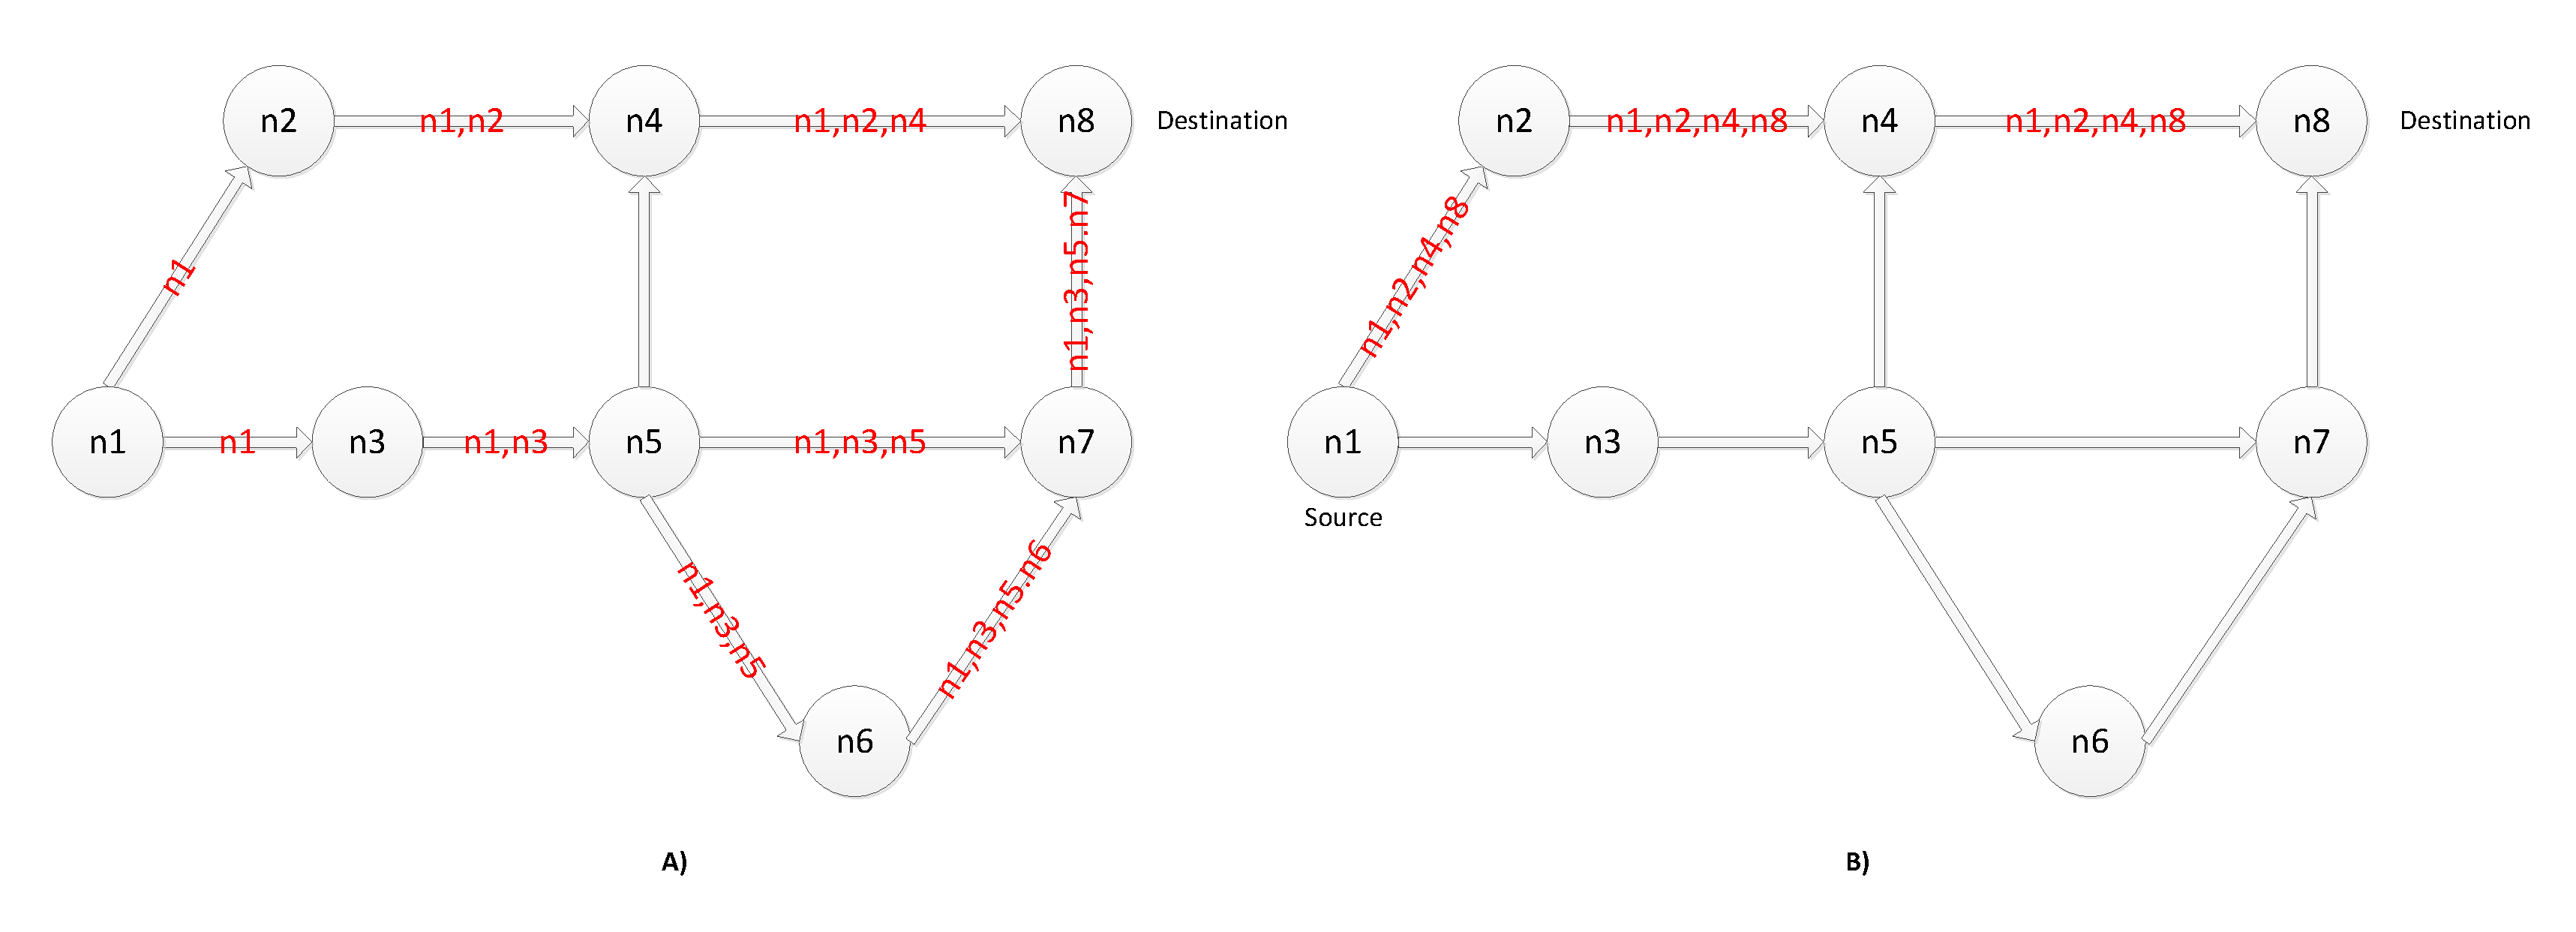
\includegraphics [height=7cm] {DSR}
\caption{Dynamic Source Routing. A) Route Discovery  B) Route Maintenance}
\label{fig:dsrFigure}
\end{figure}

In \cite{PratibhaKevre2014} an evaluation of DSR together with AODV in a grid based cluster network is  performed. For this purpose, Qualnet 5.0.2 simulator was used to excecute the performance analysis. A total of 33 nodes are deployed in an area of 1500m x 1500m. The evaluation considered the following performance metrics: i) energy consumed in transmission mode; ii) energy consumed in received mode; iii)  energy consumed in idle mode; and iv) residual battery capacity (remaining battery after simulation). Regarding the first three metrics, AODV shows a better consumption of energy that DSR (0.1 mWh vs. 0.3 mWh in the transmission mode, 0.1 mWh vs 0.3 mWh in the received mode, and 1 mWh vs. 2.5 mWh in the idle mode).  The residual battery capacity shows similar values for both protocos (around 99.7 mAhr). 

\subsection{DADR}\label{dadr}

Distributed Autonomous Depth-First Routing (DADR) \cite{Iwao2009} is a proactive distance vector protocol that uses a control mechanism to provide at most \textit{k} (if available) paths for each destination. It also utilizes Depth First Search algorithm for path recovery in cases of link failures \cite{Cespedes2012}. As the data forwarding occurs, all the information learned is used to update the routing table. This happens during periodic Hello Messages exchanged among neighboring nodes, or when the nodes receive a route poisoning message. In order to control and detect loops, a unique FID (Frame ID) is added to a packet. Each time a node forwards a packet, its FID is stored, together with the packet's sender and the packet's next hop. The FID is useful for loop detection, so that when a loop is detected, a poisoning message is generated and the other nodes in the topology are informed about the situation.

A simulation scenario of more than two thousand smart meters is presented in \cite{Iwao2010}. The authors present an analysis of the routing protocol while it is tested in a 1500-node network topology. As for adaptability, the protocol shows the capability of learning new routes in both indoor and outdoor environments. In addition, the protocol demonstrated it does not need too much control overhead when updating routes, which is an advantage in a large-scale network. The study also shows that packet latency in a flat mesh network is affected by the several hops that data packets need to traverse in order to reach the destination.

\subsection{HYDRO}\label{hydro}


Hybrid Routing Protocol \cite{Dawson2010} is a link state routing protocol for Low Power and Lossy Networks. It uses DAGs to provide multiple reliable paths to a border router. To this end, each node builds its default route table by adding its neighboring nodes toward a border router. The entries in the route table will be ordered following an ETX metric. According to the top ranked entries of its default table, each node periodically creates a topology report. The nodes piggyback the topology reports on periodic collection traffic, allowing border routers to build and maintain a global view of the topology. The first primitive of HYDRO is the provision of a Default Route Table, which is made of a list of entries (each containing the link-layer address of a node in the direction of a border router). Thus, each node has information about the link-layer packet success rates, so an evaluation of the quality of that link can be performed. This feature is especially important to fulfill the reliability, as multiple routes are provided to a given destination. HYDRO is considered both a centralized and distributed forward mechanism: on the one hand, the low-power nodes maintain a distributed DAG that provides the set of default routes for communicating with border routers; on the other hand, the border routers maintain a global view of the network topology, through the reports sent by each node. 

In \cite{Dawson2010}, a performance evaluation of HYDRO with different metrics is presented. It involves the implementation of a set of testbeds and a real network deployment. In the latter, a 57-node network was run for six months, with HYDRO as the routing protocol. The offered load consisted of each node transmitting a packet to an external server every minute. The statistics collected showed that the PDR is an average 98.9\%. As for the scalability, every node's state is bound by the number of destinations it communicates with. 

\subsection{HWMP}\label{hwmp}

The Hybrid Wireless Mesh Protocol (HWMP) is the multihop default routing protocol for IEEE 802.11s WLAN mesh networking. With the purpose of allowing interoperability between devices from different vendors, HWMP serves as a common path selection protocol for every IEEE 802.11s-compliant device. The term hybrid is due to the use of both reactive and proactive approaches in the routing scheme. HWMP results from an adaptation of AODV called Radio-Metric AODV (RM-AODV), which, unlike AODV, works on layer 2 and uses a radio-aware routing metric. 

When a node needs a path to a given destination, it broadcasts a route request message requesting a route to that destination \cite{Bahr2006}. This route request message is processed and forwarded by all mesh points to the originator of the route discovery. The destination node, or an intermediate node that owns a path to the destination, answers with a unicast reply message indicating the route requested. After this, the forward path to the destination is set up. 

Considering the diverse nature of applications that generate traffic throughout the network, and given that applying a same retransmission mechanism for all packets may reduce the network trhoughput \cite{Meng2014}, a new method of selective retransmission has been proposed. Jung \textit{et al.} \cite{Jung2011} considered the use of HWMP in a smart grid deployment, utilizing the air cost (failure rate of each node calculated by MAC retransmission count of each packet) as a performance metric. The new method gives more priority to retransmission of small packets, as they are likely to have fewer bit errors. As a conseuence, the protocol becomes more adapted for the NAN domain and the applications that are part of that architecture. 


\section{Comparison of routing protocols in AMI networks}\label{metrics}

The communication infrastructure in AMI involves an important exchange of information, which is the foundation for the location-distributed electric power devices to work in a coordinated manner. Unsatisfactory communication performance not only limits the AMI from achieving its full energy efficiency and service quality, but also poses potential damages to the grid system. To protect the AMI and ensure optimal operation, the communication infrastructure must meet a number of requirements.

In this section we compare, based on a set of selected metrics, the routing protocols for NAN environments in AMI networks introduced in Section \ref{routing}. We employ the description of operation, as well as the performance results reported in the literature to classify the protocols. The metrics employed for comparison are introduced as follows:

\subsection{Comparison Metrics}

\subsubsection{Routing strategy}
Depending on the layer in which the routing decision takes place, the data forwarding mechanisms can be classified as route-over or mesh-under. 

\begin{itemize}
\item Route-over: In a route-over scheme, all routing decisions are taken in the network layer where each node acts as an IP router. In route-over, each link layer hop is an IP hop. The IP routing supports the forwarding of packets between these links. In the forwarding process, IP routing tables and hop-by-hop options are used. For routing and forwarding processes, the network layer makes decisions using the information encapsulated in the IP header. The adaptation layer of 6LoWPAN establishes a direct mapping between the frame and the IP headers. When an IP packet is fragmented by the adaptation layer, fragments are sent to the next hop based on the routing table information. The adaptation layer of the next hop checks received fragments. If all fragments are received successfully, the adaptation layer creates an IP packet from fragments and sends it to the network layer. If the packet is destined for itself, the network layer sends the IP packet to the transport layer, otherwise forwards the packet to the next hop based on the routing table information. If there are one or more fragments missing, then all fragments are retransmitted to one hop distance. After receiving all fragments successfully the adaptation layer creates an IP packet from these fragments and passes it to the network layer. The network layer then forwards or processes the IP packet based on the destination of the packet.

\item Mesh-under: In this scheme, the network layer does not perform any IP routing. The forwarding decision is made at the adaptation layer which forwards the packet to the destination over multiple radio hops. In Mesh-Under scheme, routing and forwarding are performed at link layer based on 802.15.4 frame. To send a packet to a particular destination, 64 bit address or the 16 bit short address is used and sent it to a neighbor node to move the packet closer to the destination. Because multiple hops based on link layers are used to complete a single IP hop, it is called the mesh-under approach. An IP packet is fragmented by the adaptation layer to a number of fragments. On the other hand, these fragments are delivered to the next hop by mesh routing to reach the destination. Different fragments of an IP packet can go through different paths and they are all gathered at the destination. If all fragments are reached successfully, then the reassembling of the IP packet takes place at the adaptation laye. In case of loss of any fragment, the entire IP packet (this is, all fragments for this IP packet) must be retransmitted to the destination for recovery.
\end{itemize}

\subsection{Latency}

The concept of latency refers to the maximum time in which a particular message should reach its destination through a communication network. It is important to state that the messages between various entities within the AMI may have different network latency requirements. Thus, while commands exchanged between devices in the distribution network may require lower latency values, information exchanged between sensors and control centers may accept higher values. In \cite{Xu2011} two limit value for latency are specified, on the basis of the components that generate the traffic. As for the Phase Measurement Units (PMU) and Control Centres, 10ms is considered as the limit for an accpepted value of latency.  Regarding the AMI, and considering a reporting rate less than 1 Hz, accepted latency is under 1s.

The messages exchanged can be event driven (e.g., protection and control related) or periodic (e.g., monitoring related) \cite{Winter2012}. The network architecture and communication medium must support the diverse requirements. The network architecture will determine if the message sent from one communicating entity to the other will reach its destination in one or more hops. This will directly affect the latency. Similarly, the data rates supported by the communication medium also dictate how fast an entity can communicate an event observed or reply to a message received.  The communication technology employed should be able to provide low-latency communications from the data generation or collection point to the eventual destination. Control commands from grid operators should similarly reach smart meters and consumers with minimal delay. For the AMI application, a higher latency may be tolerable for the data collected from smart meters to the control center, but there are control commands in the other direction (from the control center to smart meters) for controlling loads and remote connect/disconnect that may needto communicate immediately.

\subsection{Availability}

 This metric indicates if the network services are available and will survive possible attacks or failures that could occur. In the HAN scenario, for example, resource depletion is typically not a concern when it comes to a resource such as energy, where both the smart meter and appliances are assumed to have access to the grid power. But computation capabilities and memory constraints could be exploited by keeping these resources fully loaded, affecting the ability of the network to function as desired. Equipment failures may also be more common, especially with the low cost of HAN radio (like the ones provided by ZigBee).

\subsubsection{Data delivery priority}
This refers to the priority of arrival of packets throughout the network, and it depends on the needs of the application. The priority may be decided at the time of connection establishment between two applications. Different levels of data delivery priority can be considered, as following: i) high, it is used where the confirmation of end-to-end data delivery is a must and a retry will be mandatory in case of absence of confirmation; ii) medium which is used where end-to-end confirmation is not required but the receiver is able to detect data loss; iii) non-critical, which is used when data loss is acceptable to the receiver. In the latter case, reliability can be improved by means of repetitive messages. The non-critical level can be used for periodic data employed for monitoring purposes. 

\subsubsection{Reliability}
The grid stability will depend, to a great extent, on the reliability of the distribution network. Hence, it becomes extremely important for the communication backbone to be reliable, in order to enable successful and timely messages exchange. Different events may affect the communication backbone reliability. Some of these failures include time-out failures, network failures, and resource failures. A time-out failure occurs if the time spent in detecting, assembling, delivering and taking action in response to a control message exceeds the timing requirements \cite{Wang2011a}.  A network failure occurs when there is a failure in one of the layers of the protocol suite employed for communication (i.e., the failure may be originated in a logical level, and it prevents packets from reaching their destination although the physical link is operative). Other factors can affect the communication, such as noise and interference. A resource failure means that one end node (i.e., sender or receiver) has failed. One of the mechanisms utilized for reliability measurements purposed is through the Packet Delivery Ratio (PDR), defined as the quotient between the number of packets received and the number of packets sent.

\subsubsection{Interoperability}
Interoperability of a smart grid is the ability of diverse systems to work together, use the compatible parts, exchange information or equipment from each other, and work cooperatively to perform tasks. It enables integration, effective cooperation, and the two-way communications proposed in the AMI concept, among the many interconnected elements of the smart grid. The NIST, which works as the first International Coordinator for smart grid interoperability, developed a framework that includes protocols and standards for information management to achieve interoperability of smart grid devices and system.


\subsubsection{Scalability}
This metric can be considered as the ability of a system to handle increasing amounts of work in an efficient manner \cite{Zhou2012}. Most of the time, the concern lies on the load scalability, which is the easiness for a system to increase its resources to accommodate the increasing load. For this purpose, it is necessary to define the specific requirements for scalability in this dimension. In the AMI case, scalability is related to the ability of the routing table on a router (meter) to scale with the number of nodes in the AMI network. Another form of scalability is related to the costs associated to the deployment of the network when the number of nodes becomes large. It is expected for the communication architecture to work equally well for a small network as well as for a large network.


\subsubsection{Ease of deployment}
This refers to the level of feasibility and easiness with which the network can be deployed. 


\subsubsection{Adaptability}
This refers to the ability of a routing protocol to adapt to different network topologies. 

\subsection{Discussion}

In \cite{Iyer2011a} a performance analysis of RPL and Geographic Routing in a Smart Grid context was executed, utilizing OMNeT++ as the simulation tool to implement the routing algorithms. Simulation were run for 500 node AMI scenarios, which were configured for gathering statistics of hop count and end-to-end delay. 

The test case used for the performance analysis was constructed based on the scenario that each of the 500 nodes sends multi-point to point traffic directed towards the collector. The application packet rate was set at 1 packet/second. All other nodes in the network simply participated in the routing and were not allowed to transmit when one of the nodes was transmitting. Each node transmitted 100 packets with the collector as the destination. An average of 160ms and 173ms of end-to-end delay were obtained for RPL and Geographical routing, respectively. 

Regarding reliability, it was measured by computing the PDR, defined as the total number of received packets at the collector over the total number of packets transmitted by each node. On this matter, RPL showed a constant packet delivery ratio between 98\% and 100\% for each packet and an average of 99.98\% while Geographical routing showed similar performance with an average of 99.30\% \cite{Iyer2011a}.  

Other protocols such as DADR and HYDRO are also analyzed, considering their behavior in testbeds and real deployments. In  \cite{Iwao2010} a study was conducted to determine the behavior of DADR in a 1500 node network topology. The study showed an average PDR of 97.8\%. HYDRO, as a combination of both centralized and distributed forwarding mechanisms, shows to have a high reliability according to \cite{Dawson2010}, as multiples routes are provided to a given destination.  By constantly evaluating the qualities of the links, the protocol becomes robust in terms of adaptability, as any change in the topology is quickly detected and the protocol reacts to it. An average PDR of 98,9\% was obtained when examining the performance of the protocol in a 57-node real deployment. 
	
A summary of the results described in this section can be observed in (Fig. \ref{fig:comparison}), where we compare the routing protocols based on the different metrics for evaluation.

\begin{figure}[h!]
\centering
\includegraphics [height=11cm] {comparativeTablev2}
\caption{Comparison of Routing Protocols in the AMI scope \cite{Wang2010} \cite{Rührup2009} \cite{Perkins2003} \cite{Toimoor2013} \cite{Johnson2007}  \cite{Dawson2010} }
\label{fig:comparison}
\end{figure}

The choice of the routing protocol may also be considered taking into account the technology that is used for deployment purposes. Thus, a protocol might fit better that other, in a certain technology. For instance, in the case of a mesh technology, a protocol that involves end-to-end retransmission when a packet loss occurs wouldn’t be too suitable, as the possibility of fragments loss is bigger in a multihop scheme.


\section{Open Networking Issues}\label{issues}

In this section, we identify the challenges related to networking issues in AMI networks. We classify them to separate the challenges inherent to the communications technology from those inherent to the routing process.

\subsection{Related to Communications Technologies}

When wireless technologies are selected for communications in the AMI, in particular in the NAN domain, aspects such as coverage, reliability, and spectrum management are still open issues \cite{Sun2012}. If coverage is increased, this may have a negative impact in terms of capacity of the wireless network, due to interference and re-transmissions caused by larger wireless links. Also, if coverage is reduced to avoid the interference problem, the number of next-hop candidates gets reduced; hence, the process of finding a path to/from the collector may fail. Relaying techniques are being proposed in order to address this trade-off between coverage and capacity \cite{Sun2012}. In terms of reliability, the extended list of applications to be supported by the AMI network brings higher standards with variable quality requirements in order to serve such applications. Nonetheless, wireless communications are susceptible to adverse weather conditions and variable propagation patterns, which directly affect the network reliability. Forwarding mechanisms that improve reliability in AMI networks with highly unstable links have been proposed to address this issue \cite{Cespedes2012}. Spectrum management is another key challenge when more and more wireless technologies over unlicensed bands are deployed. Such is the case for 802.11-based and 802.15-based technologies that are employed in the NAN domain. An efficient use of the spectrum is therefore a critical issue.

If the selection is for a wired technology, such as PLC, then network adaptability is an issue to consider. In the majority of cases, bus or star topologies that connect smart meters to a collector are employed with wired technologies. Thus, a single link failure may represent the complete disconnection of a customer premises since the nature of the technology does not permit to find alternative paths (unless redundant links are employed, which increases the deployment costs).  Another issue among the different wired technologies is the interoperability. Since Automatic Meter Reading (AMR) has been present for some time, traditional technologies employed at the time did not consider the possibility to interconnect to other networks. Most solutions are built on top of proprietary stacks of protocols that reduce the chances to re-use such technologies in order to deploy the new IP-based applications expected in the AMI network.

\subsection{Related to the Routing Process}

There are several open issues that need to be addressed together with routing. On the one hand, there is the need for securing the information that is transmitted across the smart grid. Apart from mitigation of cyber-security attacks, a balance between individual energy consumption data for billing purposes and aggregated data for statistical analysis is required from the AMI \cite{Saputro2012}. On the other hand, the different natures of traffic due to an expanded list of applications to be deployed in the AMI raises the need for QoS-aware routing. Hence, routing metrics should adapt to fulfill the QoS requirements. Although complex combinations of metrics can be achieved through objective functions such as the one proposed in RPL  \cite{Dohler2009}, there is still a lack of flexibility for the objective function to adapt ``on the fly" according to the type of traffic that is being routed at a certain time. 

Moreover, the NAN domain of an AMI network poses a critical challenge: a network with a number of nodes that start from hundreds and may grow to millions. Although scalability is defined as one of the design factors of routing protocols, those employed in the AMI context need to demonstrate that a minimum level of performance can actually be maintained in a very large network.


\section{Conclusion}\label{conclusion}

In this paper, we have presented a comprehensive survey of communication technologies and routing protocols for Advance Metering Infrastructure deployments, with a special focus on the network domain that connects the smart meters at customer premises and data collectors that connect to the utility, namely the Neighborhood Area Networks (NAN) in AMI. We have described the evolution of the AMI network and the advances in real deployments around the world. As for the communication technologies, we have provided a classification of the different wired and wireless options, identifying the network domain in which each technology fits better. Together with the communication technologies, we have also provided descriptions for the routing protocols proposed for the NAN domain and the set of metrics we have employed for the comparison. Open networking issues are also provided and classified depending on whether they are related to the communication technology or the routing process. A proper balance between coverage and capacity are aspects to be investigated when employing wireless technologies for a NAN network with a large number of nodes. Also, while legacy Automated Meter Reading (AMR) systems can be extended to support other AMI applications, interoperability is still an issue, specially when connection to traditional IP networks is expected. Aspects such as secure routing, privacy protection, and QoS capabilities need further study for routing in the NAN domain to support the extended list of applications to be supported in the AMI network. 


%\appendices
%\section{Proof of the First Zonklar Equation}
%Appendix one text goes here.
%
%% you can choose not to have a title for an appendix
%% if you want by leaving the argument blank
%\section{}
%Appendix two text goes here.
%
%
%% use section* for acknowledgement
%\section*{Acknowledgment}
%
%
%The authors would like to thank...


% Can use something like this to put references on a page
% by themselves when using endfloat and the captionsoff option.
\ifCLASSOPTIONcaptionsoff
  \newpage
\fi



% trigger a \newpage just before the given reference
% number - used to balance the columns on the last page
% adjust value as needed - may need to be readjusted if
% the document is modified later
%\IEEEtriggeratref{8}
% The "triggered" command can be changed if desired:
%\IEEEtriggercmd{\enlargethispage{-5in}}

%references section

% can use a bibliography generated by BibTeX as a .bbl file
% BibTeX documentation can be easily obtained at:
% http://www.ctan.org/tex-archive/biblio/bibtex/contrib/doc/
% The IEEEtran BibTeX style support page is at:
% http://www.michaelshell.org/tex/ieeetran/bibtex/
\bibliography{bibliography_ami_final}
\bibliographystyle{IEEEtran}
% argument is your BibTeX string definitions and bibliography database(s)
%\bibliography{IEEEabrv,../bib/paper}a
%
% <OR> manually copy in the resultant .bbl file
% set second argument of \begin to the number of references
% (used to reserve space for the reference number labels box)
%\bibliographystyle{ieeetr}
%\bibliography{IEEEabrv,}

% biography section
%
% If you have an EPS/PDF photo (graphicx package needed) extra braces are
% needed around the contents of the optional argument to biography to prevent
% the LaTeX parser from getting confused when it sees the complicated
% \includegraphics command within an optional argument. (You could create
% your own custom macro containing the \includegraphics command to make things
% simpler here.)
%\begin{biography}[{\includegraphics[width=1in,height=1.25in,clip,keepaspectratio]{mshell}}]{Michael Shell}
% or if you just want to reserve a space for a photo:

%\begin{IEEEbiography}{Michael Shell}
%Biography text here.
%\end{IEEEbiography}
%
%% if you will not have a photo at all:
%\begin{IEEEbiographynophoto}{John Doe}
%Biography text here.
%\end{IEEEbiographynophoto}

% insert where needed to balance the two columns on the last page with
% biographies
%\newpage

%\begin{IEEEbiographynophoto}{Jane Doe}
%Biography text here.
%\end{IEEEbiographynophoto}

% You can push biographies down or up by placing
% a \vfill before or after them. The appropriate
% use of \vfill depends on what kind of text is
% on the last page and whether or not the columns
% are being equalized.

%\vfill

% Can be used to pull up biographies so that the bottom of the last one
% is flush with the other column.
%\enlargethispage{-5in}



% that's all folks
\end{document}


